\subsection*{research}
i discovered \autocite{rf-amp-classics} (see \localfile{../research/books/}),
an \arrl book on \rf amplifiers, and skimmed through it. some items of
interest:
\begin{enumerate}
	\item \autocite[p.~1 dash 41]{rf-amp-classics}: class-E power
	amplifiers are a highly power- and parts-efficient amplifier topology,
	utilizing a single active element and a tuned load. the article,
	``High-Efficiency Class-E Power Amplifiers,'' claims 21-fold power
	improvement over class-A for a given dissipated power. since our
	fractional bandwidth is not that high (\textasciitilde 2.5 \%), we
	could get away with a Q of 40 in the tuned load and still transmit
	across the band, so class-E might be feasible! the circuit used in the
	article is reproduced in figure \ref{fig:class-e-from-article}.

	\begin{figure}[H]
		\centering
		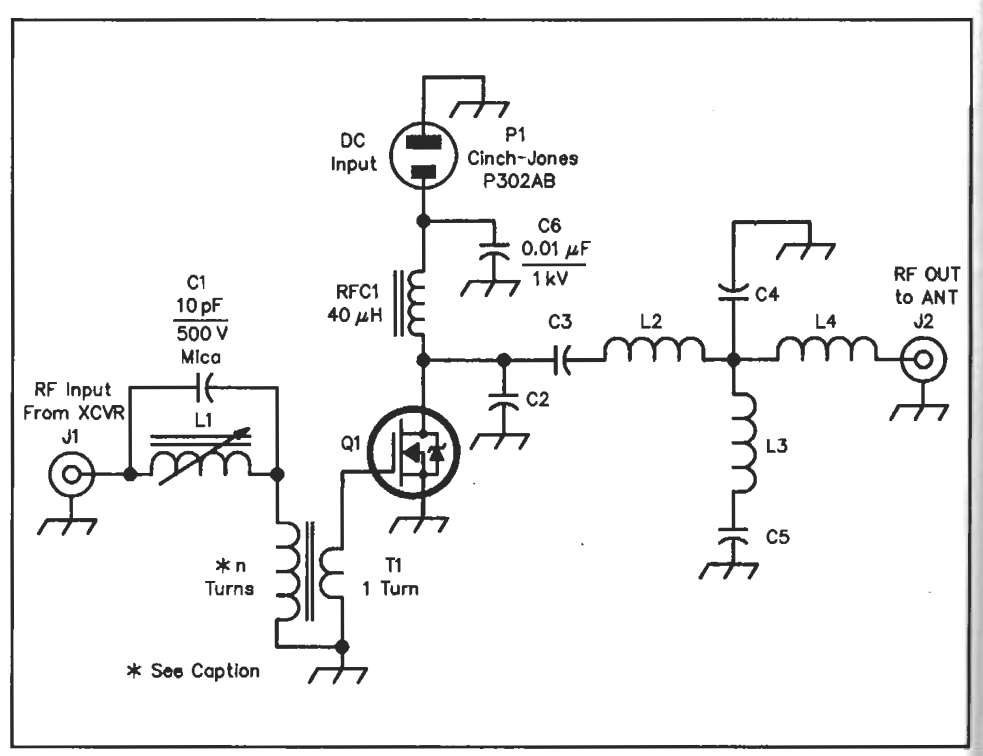
\includegraphics[width=.7\textwidth]{class-e-from-article.png}
		\caption{a class-E amplifier.}
		\label{fig:class-e-from-article}
	\end{figure}

	i have a slight advantage in that i know about these amplifiers from
	elsewhere\ldots\ but here's how they work anyway: the load network
	comprising \pr{c2, c3, c4, c5, l2, l3, \amp l4} (basically everything
	hanging off \pr q1's drain) is resonant somewhere near the transmission
	frequency. the network is carefully damped, so that when \pr q1
	switches off, the voltage across it rises, then neatly falls back to
	zero just by the next turn-on. figure \ref{fig:class-e-vi}, also from
	the article, shows this. some of \pr q1's drain network also filters
	the output so the amp doesn't pollute the spectrum.

	\begin{figure}[H]
		\centering
		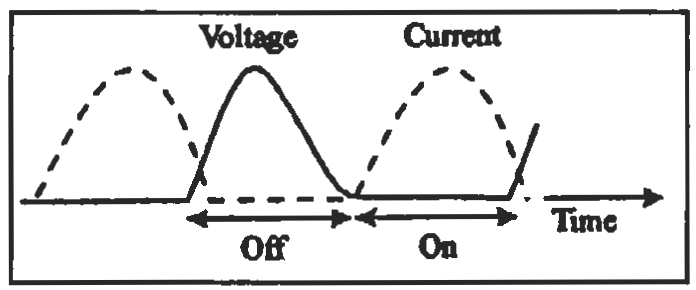
\includegraphics[width=.7\textwidth]{class-e-vi.png}
		\caption{class-E voltage \amp current.}
		\label{fig:class-e-vi}
	\end{figure}

	\item \autocite[p.~2 dash 5]{rf-amp-classics}: this article, ``A 300-W
	MOSFET Linear Amplifier for 50 MHz,'' contains another amplifier
	topology: the push-pull kind. its schematic is reproduced in figure
	\ref{fig:push-pull-article}.

	\begin{figure}[H]
		\centering
		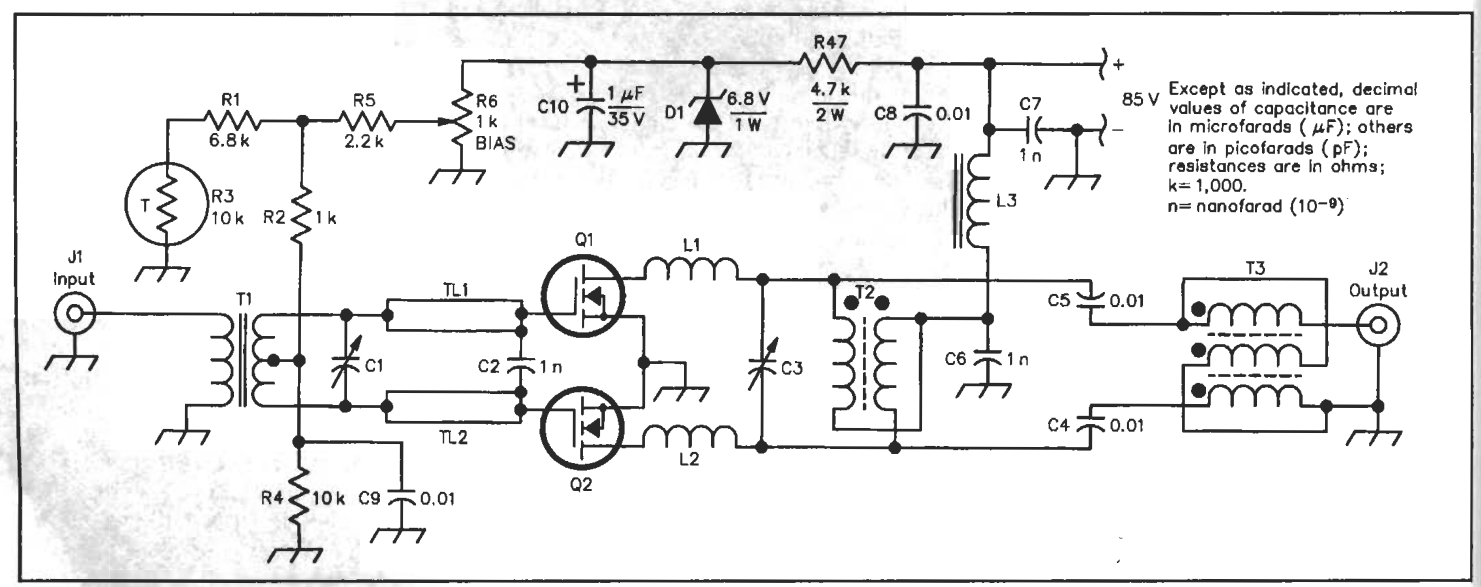
\includegraphics[width=.9\textwidth]{push-pull-article.png}
		\caption{push-pull amplifier schematic.}
		\label{fig:push-pull-article}
	\end{figure}

	the article does not describe how this amplifier works in detail. as
	far as i can tell: \pr t1 feeds \pr q1 \amp \pr q2 with precisely
	out-of-phase drive signals through matching transmission line segments
	\pr{tl1 \amp tl2} (chosen to impedance-match their gates to whatever
	the input transformer impedance is). \pr q1 \amp \pr q2 feed \pr t2
	\amp \pr t3, drawing out-of-phase current pulses from \pr t2 to produce
	an \rf signal out at \pr j2.

	notably, the efficiency claimed by this article is \textasciitilde 50\%
	at most, much less than the 90 \% efficiency of class-E.

	\item \autocite[p.~1 dash 2]{rf-amp-classics}: ``An Easy-to-Build
	25-Watt MF/HF Amplifier'' contains a push-pull amp which is
	significantly easier to understand! part of its schematic is reproduced
	in figure \ref{fig:easy-hf-article}.

	\begin{figure}[H]
		\centering
		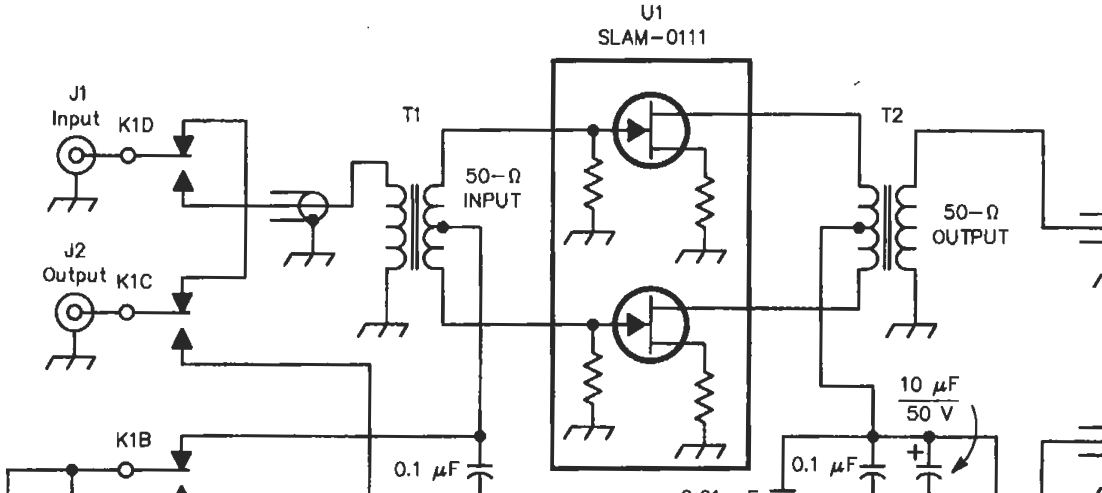
\includegraphics[width=.8\textwidth]{easy-hf-article.png}
		\caption{an easier push-pull amplifier.}
		\label{fig:easy-hf-article}
	\end{figure}

	it seems that\ldots\ \pr t1 converts a single-ended input signal into a
	differential signal, which is used to feed the dual-\jfet block \pr u1.
	each \jfet produces a signal exactly out of phase with the other, which
	are fed into opposite ends of \pr t2's primary winding. each \jfet will
	then cause \pr t2's output to swing positive or negative, resulting in
	an amplified input signal.

	the output of the amplifier is then fed into a switchable low-pass lc
	filter network, presumably to eliminate higher-order harmonics in its
	output. this amplifier is, notably, a \emph{broadband} one!

	\item \autocite[p.~1 dash 19]{rf-amp-classics}: ``A 1.8 to 54 MHz
	5-Watt Amplifier'' uses a much simpler (and probably less efficient)
	topology than either of the above, using simply a single \mosfet
	class-A with an inductive choke as the load. the schematic is
	reproduced in figure \ref{fig:five-watt-article}.

	\begin{figure}[H]
		\centering
		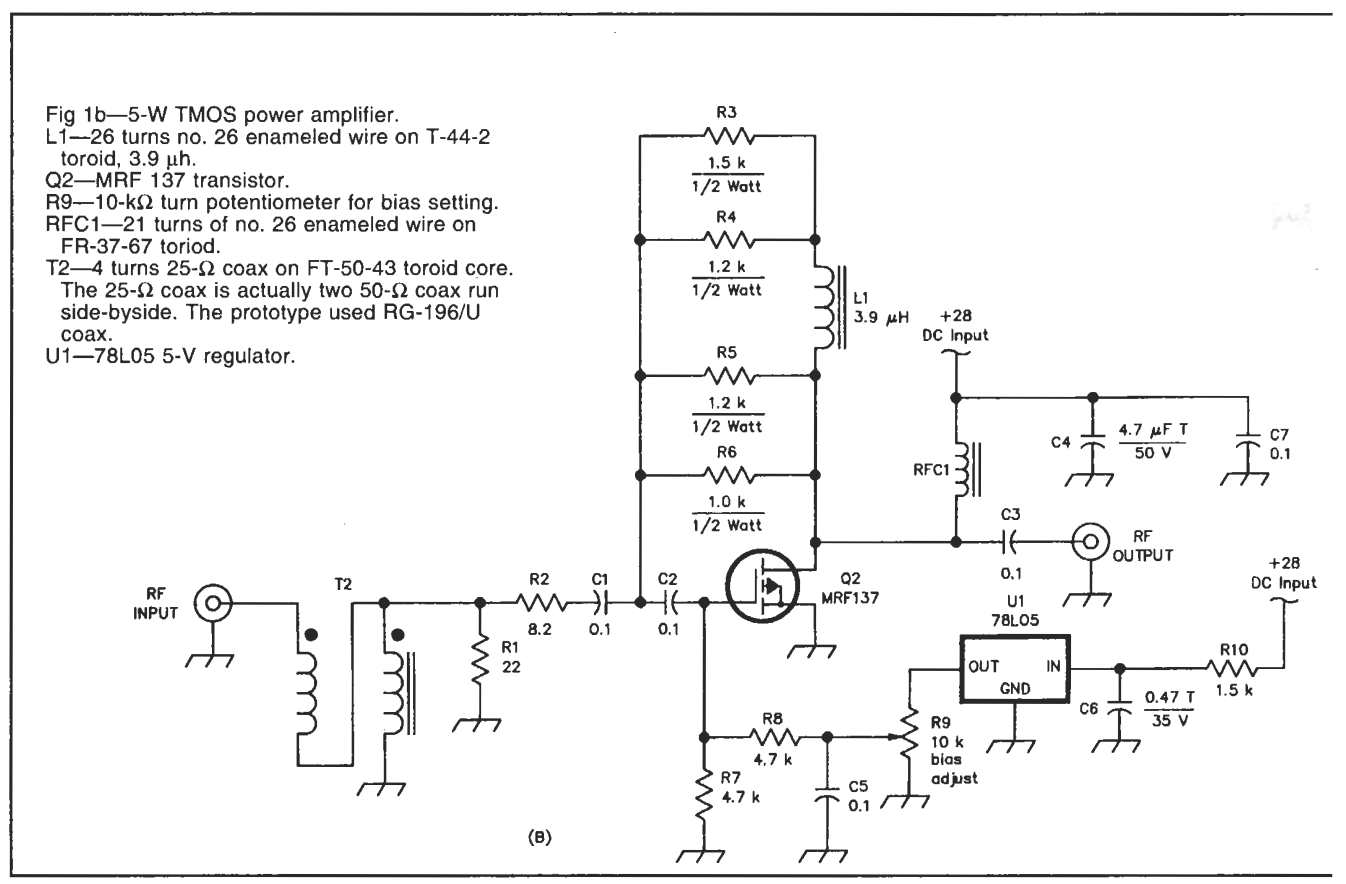
\includegraphics[width=.9\textwidth]{five-watt-article.png}
		\caption{a class-A linear amplifier.}
		\label{fig:five-watt-article}
	\end{figure}

	the essential components of this amplifier are \pr q2 and \pr{rfc1},
	which form a current source against a very high impedance at signal
	frequencies. this is probably the simplest \rf amplifier design, and
	likely the one that we'll use for low- and intermediate-power stages
	since it's easy and linear.
\end{enumerate}

in addition to the above, i also skimmed razavi's chapter in
\autocite{rf-microelectronics} (same place, \localfile{../research/books/}) on
phase-locked loops for inspiration about generating a reference frequency. if
we are not to get in trouble with the \fcc, we'll need a stable oscillator. my
idea right now is to use a \textasciitilde 50 kHz local crystal oscillator with
a \pll to increase its frequency in 50 kHz steps around 14 MHz, which should
give stability in the single Hz (averaged) and tunability.

\subsection*{code}
i typeset this log and wrote the first two entries.
